%%%%%%%%%%%%%%%%%%%%%%%%%%%%%%%%%%%%%%%%%%%%%%%%%%%%%%%%%%%%%%%%%
% Dissertacao de Mestrado / Dept Fisica, CFM, UFSC              %
% Lacerda@UFSC - 2013                                           %
%%%%%%%%%%%%%%%%%%%%%%%%%%%%%%%%%%%%%%%%%%%%%%%%%%%%%%%%%%%%%%%%%

%:::::::::::::::::::::::::::::::::::::::::::::::::::::::::::::::%
%                                                               %
%                          Capítulo 1                           %
%                                                               %
%:::::::::::::::::::::::::::::::::::::::::::::::::::::::::::::::%

%***************************************************************%
%                                                               %
%                         Introdução                            %
%                                                               %
%***************************************************************%

\chapter{Introdução}
\label{sec:Intro}

%***************************************************************%
%                                                               %
%              Introdução - Um labirinto de dados               %
%                                                               %
%***************************************************************%

\section{Um labirinto de dados}
\label{sec:Intro:LabData}

Cientistas hoje, em sua maioria, encontram-se emaranhados em meio a um labirinto de informações. Grandes corredores com
bilhões de intersecções interligadas que funcionam como uma fantástica e infinita biblioteca de dados. Um dia formada
por livros, hoje formada de 0s e 1s que juntos, através de um número interminável de combinações, abarcam o combustível
para o desenvolvimento do conhecimento da humanidade. Qualquer que seja sua área, você tem, já teve, ou terá um dia que
recorrer a algum banco de dados de qualquer espécie pois hoje são parte fundamental no futuro da pesquisa científica. Na
Astrofísica tais informações hoje são reunidas através de grandes projetos chamados {\em surveys}.

Um {\em survey} astronômico é um levantamento de informações ou mapeamento de regiões do céu utilizando telescópios e
detetores. Primordialmente surgem com a inata curiosidade do homem de observar e registrar tudo à sua volta. O
crescimento desses catálogos é produto direto da evolução dos equipamentos usados nestas investigações. No início da
década de 80, \citet{Huchra1983} constroem um {\em redshift-survey} que coletou espectros para 2500 galaxias dando
início a produção sistemática de dados na astronomia extragalática. Esse trabalho foi seguidos por outros \citep[e.g.,
][]{Huchra1988, DaCosta1988} e de lá para cá a quantidade (e a qualidade) de dados só aumentou. Com a criação dos {\em
mega-surveys} \citep[\SDSS, 2dFGRS, 2MASS; ][]{York2000, Colless1999, Skrutskie2006}, alguns já terminados, outros ainda
começando ou por terminar \citep[LSST, JPAS; ][]{Ivezic2008, Benitez2009}, ultrapassou-se o patamar do humanamente
impossível de se analisar individualmente cada objeto, necessitando assim a ajuda de máquinas e métodos computacionais
cada vez mais eficientes. Com esse crescimento exponencial na quantidade de dados, precisamos cada vez mais de
ferramentas matemáticas/estatísticas, e essa dissertação trata precisamente disso.

Um tipo de clássico de ferramenta de análise são os programas que ajustam os dados segundo algum modelo, extraíndo dessa
análise informações de valor astrofísico. No contexto de espectros de galáxias, tema desta dissertação, uma ferramenta
deste estilo é o código \starlight, desenvolvido por \citet{CidFernandes2005}, que decompõe o espectro observado em
termos de populações estelares de distintas idades e metalicidades em um processo conhecido como síntese espectral.
A aplicação desse método a quase um milhão de espectros de galáxias do \SDSS gerou uma série de resultados \citep[e.g.,
][]{Asari2007, Asari2009, CidFernandes2007, Mateus2007}. O \starlight, assim como várias outras ferramentas similares
\citep{Panter2003, Gallazzi2005, Ocvirk2006} propõe uma pergunta bem definida (``qual a história de formação de
uma dada galáxia'') e a respondem através de parâmetros extraídos do ajuste dos dados (i.e., da síntese espectral). O
mapeamento do espaço de observáveis em um espaço de parâmetros envolve uma série de questões matemáticas e estatísticas
complexas. Mesmo assim, este método é essencialmente calcado em princípios físicos.

Outros métodos são de natureza mais puramente matemática, buscando no espaço de dados observados estruturas e
correlações que possivelmente revelem (ou pelo menos nos dêem pistas sobre) os fenômenos subjacentes. Aqui, a pergunta é
bem definida em um sentido matemático, e o desafio é interpretar a resposta em termos físicos.
\citet{SanchezAlmeida2010}, por exemplo, categorizam espectros de galáxias do \SDSS/DR7 em termos de {\em clusters}
formados pelas distâncias euclidianas entre os pontos formados pelo espectro de cada galáxia em um espaço de dimensão
$N_\lambda$. Cada cluster desse foi caracterizado por um espectro médio chamado de {\em K-mean} e é usado para posterior
comparação com outros espectros. 

Um método bem mais popular e tradicional nessa mesma linha é a análise de componentes principais (PCA - {\em Principal
Component Analisys}). A técnica de PCA é simples, não-paramétrica, e nos ajuda a extrair informações de conjuntos de
dados com muitas variáveis. Resumidamente, a PCA parte de uma tabela de $N$ linhas (objetos) por $M$ colunas (contendo
propriedades observadas para cada objeto) e reorganiza as colunas transformando as propriedades originais em combinações
delas mesmas de forma que as diferenças (a variância) entre os objetos  esteja concentrada nas primeiras colunas,
reduzindo assim dimensionalidade do problema (mais detalhes em \ref{sec:PCAeTomoPCA:PCA}). A tabela pode conter
quaisquer tipos de dados, como cores, tamanho, dispersão de velocidade, luminosidade, etc. No caso de espectros de
diferentes galáxias \citep[e.g., ][]{Francis1992, Sodre1994, Sodre1997}, as propriedades são as medidas de fluxo para
cada comprimento de onda: $F_{gl} = F_g(\lambda_l)$, com $l = 1 \ldots M$ comprimentos de onda, para cada galáxia $g = 1
\ldots N$.

Hoje, PCA é utilizada exaustivamente em várias áreas de conhecimento, principalmente em reconhecimento de padrões,
computação visual, filtragem e compactação de dados \citep{Kamruzzaman2010, Borcea2012}. Podemos ver exemplos também em
medicina \citep{Balakrishnan2013}. Na Astrofísica o PCA passeia por diversas ramificações da área. A luz de um objeto
até nossos telescópios sofre influência de ruído e é afetada pela atenuação e avermelhamento por poeira, contaminação
ótica através de objetos que estejam no mesmo campo, entre outros. Os próprios instrumentos também geram diversas
assinaturas indesejadas. Por todos esses motivos fica claro que os dados geralmente necessitam de uma boa filtragem.
Junto com outras técnicas (tomogramas, wavelets, Fourier), o PCA vem sendo muito utilizado para filtragem de dados,
principalmente cubos de dados advindos de IFS que possuem muitas dessas assinaturas instrumentais \citep{Riffel2011}.
Outro exemplo de uso de PCA aparece no artigo IV do grupo SEAGal/\starlight \citep{Mateus2007} auxiliando no estudo da
dependência ambiental de algumas propriedades físicas (idade estelar média ponderada pela luz, massa estelar,
metalicidade estelar e razão massa/luminosidade) em uma amostra de galáxias do \SDSS/DR4. Em \citet{Chen2012} é criada
uma biblioteca com $25$ mil modelos de espectros de galáxias com diferentes idades, metalicidades, velocidade de
disperção, SFH ({\em star formation history}), extinção por poeira e aplicado PCA em cima dessa biblioteca (ver Figura
\ref{fig:Chen2012fig2}). Usando uma minimização quadrática encontram quais os coeficientes e qual o número ótimo de PCs
que melhor estimam os parâmetros físicos dos espectros modelo. Então projetam os espectros observados pelo \SDSS/DR7
\citep{Abazajian2009} e pelo {\em Baryon Oscillation Spectroscopic Survey} \citep[BOSS;][]{Ahn2012}, atribuindo um
sentido físico a cada PC. Os trabalhos de \citet{Ferreras2006, Wild2006, Rogers2007} exemplificam outras aplicações de
PCA a espectros do \SDSS.

\begin{figure}
    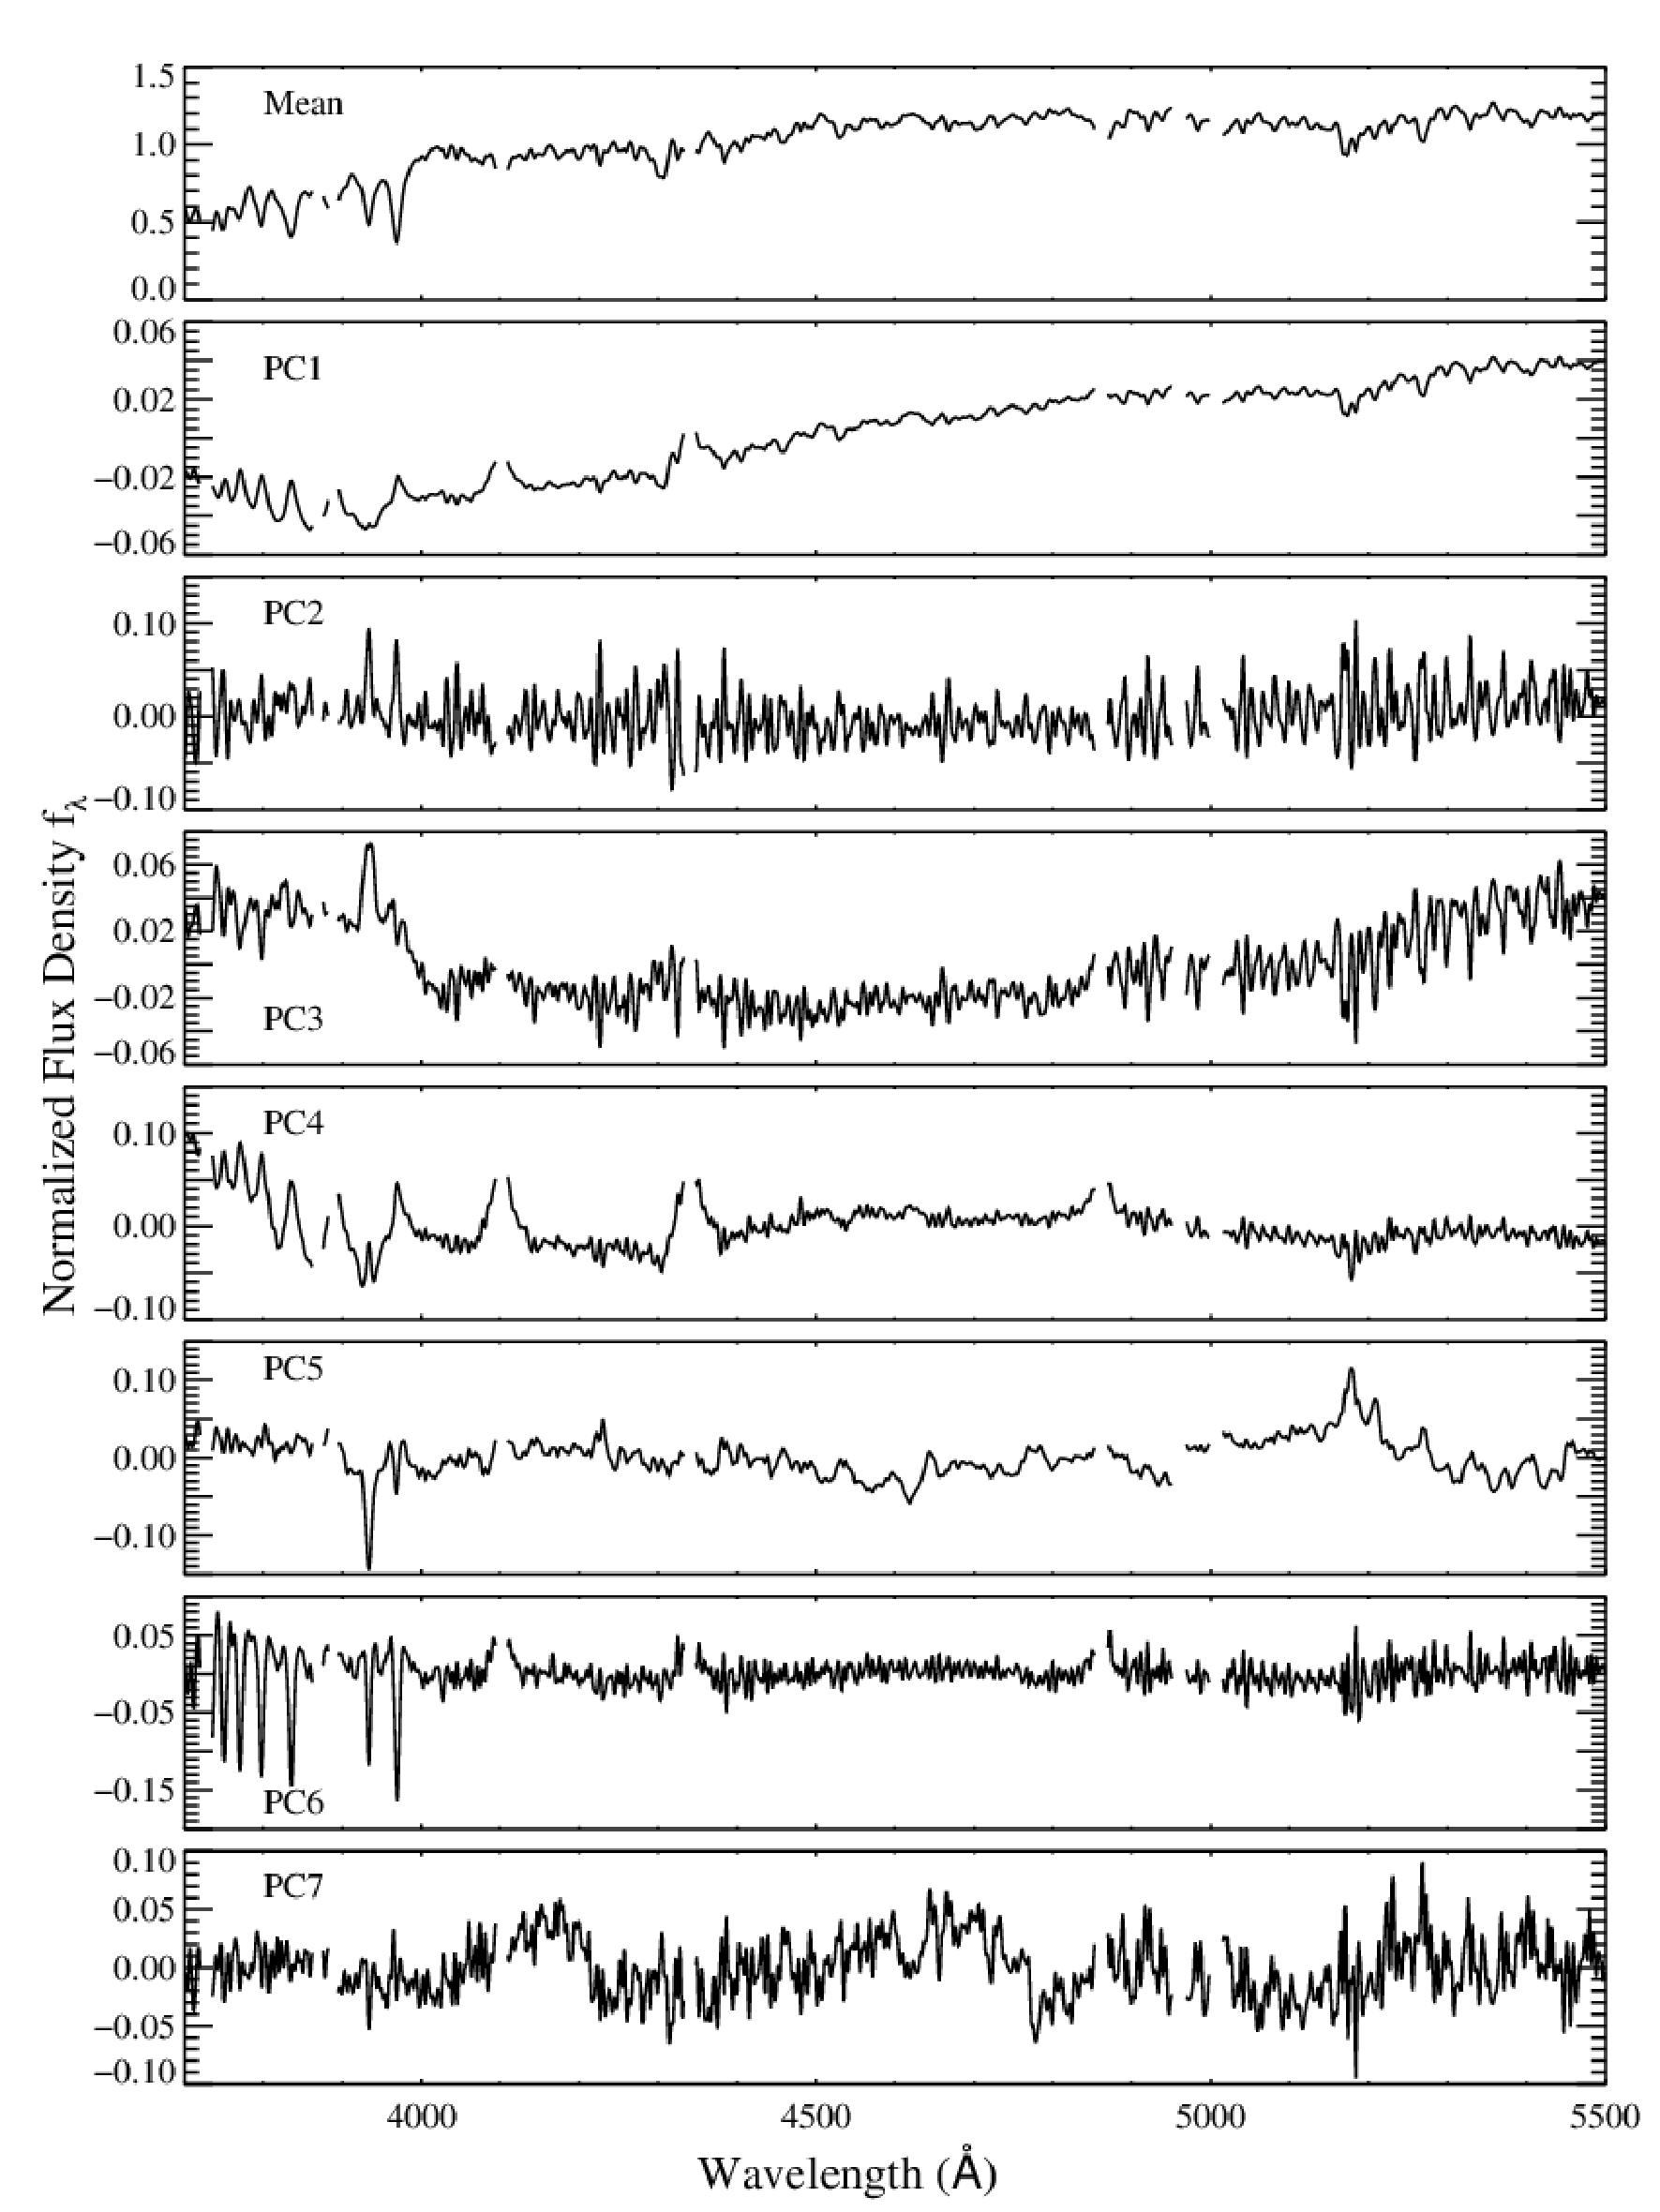
\includegraphics[height=1.\textwidth]{figuras/figChen2012fig2.pdf}
    \caption[Espectro médio e 7 primeiras PCs de uma biblioteca de modelos.]
    {De cima para baixo: O espectro médio da biblioteca de espectros modelos seguido dos sete primeiros autoespectros
    da análise PCA. Retirado de \citet{Chen2012}.}
    \label{fig:Chen2012fig2}
\end{figure}

\section{A nova ferramenta - Tomografia PCA}
\label{sec:Intro:TomoPCA}

Todos estes exemplos anteriormente citados relatam análises de espectros integrados de galáxias, i.e., espectros que
contém toda luz (ou pelo menos boa parte) da galáxia. Análises como a síntese espectral ou PCA comparam galáxias
inteiras umas com as outras, ordenando-as em termos de propriedades físicas (e.g., a massa estelar ou a idade média das
estrelas) ou matemáticas (e.g, suas componentes principais ou variâncias). Existem também exemplos de análises PCA ou de
síntese espectral baseadas em espectros nucleares \citep[e.g., ][]{Trager2000I, CidFernandes2004}. Assim como espectros
integrados, tais estudos não possuem resolução espacial, ou seja, cada galáxia é representada por apenas um espectro.

Hoje, com o uso de painéis de fibras óticas apontadas para as galáxias, temos os {\em surveys} de IFS ({\em Integral
Field Spectroscopy}) onde passamos a reunir de dezenas até milhares de espectros cobrindo um {\em FoV} ({\em
field-of-view}\footnote{Campo de visão.}) de toda uma galáxia. Assim temos para cada píxel (duas dimensões espaciais) um
espectro (uma dimensão espectral), formando assim um cubo de {\em spaxels}\footnote{spectral pixels}. Um pioneiro nessa
produção em massa de dados é o {\em Calar Alto Legacy Integral Field spectroscopy Area
survey\footnote{\url{http://www.caha.es/CALIFA/}}} \citep[CALIFA; ][]{CALIFAPresent2012}, produzindo cerca de quatro mil
espectros por galáxia observada. Outros {\em mega-surveys} IFS estão por vir (veja a seção \ref{sec:CALePyC:Apresent}).

Com esses cubos de dados, cada galáxia passa a ser uma grande amostra de espectros, de modo que o que antes era feito
galáxia a galáxia pode agora ser feito para diferentes regiões de uma mesma galáxia. Podemos assim executar o \starlight
para cada {\em spaxel} e então obtemos propriedades físicas das populações estelares em função da posição na galáxia.
Este tipo de análise vem sendo realizado por pesquisadores do Instituto de Astrofísica de Andalucía, na Espanha (IAA;
Enrique Pérez, Rosa González Delgado, Rubén García-Benito) e do Grupo de Astrofísica da Universidade Federal de Santa
Catarina (GAS-UFSC; André Luiz de Amorim, Natália Vale Asari, Roberto Cid Fernandes). Aspectos técnicos e incertezas são
discutidos em \citet[][CF13 daqui pra frente]{CidFernandes2013} e \citet{CidFernandes2014}, enquanto \citet{Perez2013},
e \citet{GonzalezDelgado2014} apresentam resultados astrofísicos dessa análise. Neste trabalho explorarenos os mesmo
dados através da técnica de PCA.

A aplicação de PCA a cubos de dados foi realizada pela primeira vez por \citet[][S09 daqui pra frente]{Steiner2009}, que
cunharam o termo Tomografia PCA. Com essa nova técnica temos, além da análise das componentes principais, uma imagem
formada pela matriz de covariância (as questões matemáticas serão abordadas no Capítulo \ref{sec:PCAeTomoPCA}). Assim
podemos saber o peso, ou relevância, de cada componente principal (daqui pra frente PC) relacionada a uma posição na
galáxia, combinando as virtudes de espectroscopia com as de imageamento.

Além de S09, outros exemplos de uso de Tomografia PCA podem ser encontrados em \citet{Riffel2011} e \citet{Ricci2011}.
Cumpre salientar que todas essas aplicações dessa nova técnica são baseadas em dados que cobrem apenas a região um campo
de $3^{\prime\prime} \times 5^{\prime\prime}$ correspondendo algumas centenas de parsecs centrais. Esta é naturalmente
uma região rica em fenomenologia e portanto interessante de ser estudada com IFS, como ilustram os próprios resultados
dos artigos supracitados (ver também Seção \ref{sec:PCAeTomoPCA:TomoPCA}).

\section{Este trabalho}
\label{sec:Intro:ThisWork}

Através da colaboração do GAS-UFSC com o grupo de pesquisadores do projeto CALIFA temos a oportunidade de trabalhar com
os dados de IFS das galáxias observadas por esse projeto, que ainda está em andamento. O seu primeiro {\em Data
Release\footnote{\url{http://www.caha.es/CALIFA/public_html/?q=content/califa-dr1}}} \citep[][DR1]{Husemann2013} possui
$100$ objetos e por volta de $400$ mil espectros. A previsão é que ao término do projeto serão observadas até $600$
objetos. Embora outros surveys de IFS estejam completos ou em andamento (ver Seção \ref{sec:CALePyC:Apresent}), o CALIFA
é o que podemos chamar de {\em estado da arte} em surveys de espectroscopia de campo integrado (IFS).

Como já citado, pesquisadores do IAA e da UFSC vêm aplicando o \starlight aos cubos do CALIFA e com isso mapeando as
propriedades das populações estelares nessas galáxias. Mais de 300 cubos de dados já foram analisados, embora os
resultados publicados até agora se restrinjam a pouco mais que 100 galáxias, de espirais tardias até elípticas,
incluindo alguns sistemas em interação. Ferramentas desenvolvidas nesses trabalhos anteriores serão utilizadas nessa
dissertação, como veremos mais adiante.

Neste trabalho aplicaremos a técnica de Tomografia PCA a alguns cubos de dados do CALIFA. O objetivo é pura e
simplesmente ver o que se obtém! Como bem colocado por \citet{Steiner2009}, o grande problema da PCA é que você tem a
resposta, mas não sabe exatamente qual é a pergunta! Este é, portanto, um estudo eminentemente exploratório, motivado
pelo sucesso dos trabalhos de Steiner e colaboradores em suas aplicações dessa nova ferramenta de análise de cubos
dados.

É importante notar, no entanto, que existe uma grande diferença entre esses trabalhos anteriores e esse estudo.  Nossos
cubos de dados cobrem uma escala completamente diferente. De fato, o CALIFA foi desenhado para observar galáxias
inteiras. O campo do instrumento utilizado é de aproximadamente 1.3 arcmin$^2$. Em comparação com os estudos de Steiner
e colaboradores, temos uma resolução espacial muito ``pior'', mas em compensação mapeamos estruturas muito diferentes,
como o bojo, disco, braços e regiões H{\sc ii} a muitos kpc do núcleo. Como veremos, esta diferença nos levou a tratar
os dados de formas que diferem daquelas empregadas por Steiner e seus colaboradores. De fato, até onde temos conhecimento,
este trabalho é o primeiro a aplicar a técnica de tomografa PCA à galáxias interias.

\subsection{Organização deste trabalho}

No seguinte capítulo apresentamos de forma resumida o {\em survey} CALIFA e dois pipelines importantes para a
organização dos dados utilizados neste trabalho: \pycasso e {\sc qbick}.

O terceiro capítulo descreve matematicamente a técnica de PCA e a Tomografia PCA, bem como sua utilização no presente trabalho. 

No quarto capítulo discutimos diferentes {\em configurações}\footnote{Configurações aqui é usado apenas como uma maneira
de tipificar diferentes pré-processamentos ou conjuntos dos dados antes da execução da PCA.} de execução da PCA,
juntamente com suas implicações aos resultados das análises. As diversas escolhas relativas à etapas de
pré-processamento dos dados são discutidas de forma exemplificada.

Com todo o arcabouço teórico em mãos, no capítulo cinco temos um estudo de caso para 8 objetos do CALIFA, escolhidos
para abarcar "de tudo um pouco". São galáxias 4 espirais, 2 {\em early-type} e 2 objetos compostos (mergers). Como
forma de compação com os resultados da síntese de populações estelares executadas pelo \starlight nesses objetos também
é feita uma espécie de engenharia reversa através de correlações e comparações.

Por fim, temos as conclusões e perspectivas futuras deste trabalho e da nossa colaboração com o projeto CALIFA no sexto
e último capítulo. 

% End of this chapter
